\part{Optimisation}
\frame{\partpage}

\begin{frame}{Optimisation}
	\begin{itemize}
		\pause\item Define a \textbf{fitness function} $f(x)$
		\pause\item $f(x)$ \textbf{evaluates} a piece of content $x$, assigning it a \textbf{numerical score}
		\pause\item \textbf{Higher} scores are \textbf{better}
		\pause\item We are exploring a \textbf{fitness landscape}
	\end{itemize}
\end{frame}

\begin{frame}{Running example}
	\begin{itemize}
		\pause\item \url{08_pathfinding} in \url{bsc_live_coding} repository
		\pause\item Want to generate a map where there is a path from start to goal,
			and that path is as long as possible
		\pause\item Fitness measure:
		$$ f(x) = \begin{cases}
			\text{path length} & \text{ if a path exists} \\
			0 & \text{ otherwise}
		\end{cases} $$
	\end{itemize}
\end{frame}

\begin{frame}{Hillclimbing (a.k.a.\ gradient ascent)}
	\begin{itemize}
		\pause\item Start with an element $x$
		\pause\item Create an element $x'$ by making a \textbf{small change} to $x$
			\begin{itemize}
				\pause\item May choose the small change at random
				\pause\item Or may try every possible change
			\end{itemize}
		\pause\item If $f(x') > f(x)$, set $x = x'$
		\pause\item Otherwise, throw $x'$ away and keep $x$ as it is
		\pause\item Repeat
	\end{itemize}
\end{frame}

\begin{frame}{Local optima}
	\pause
	\begin{center}
		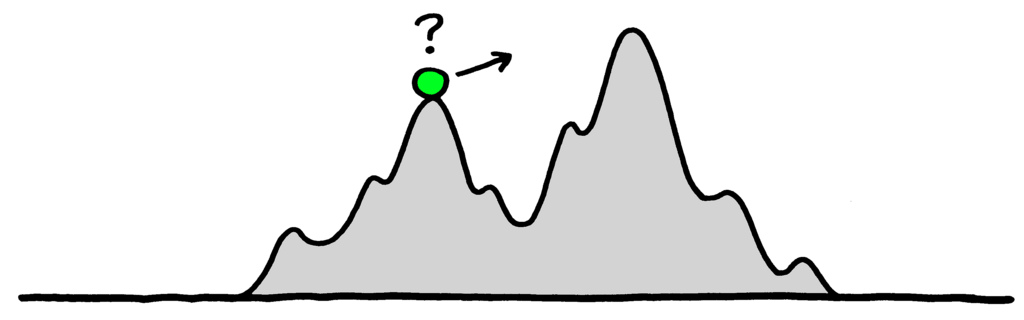
\includegraphics[width=0.6\textwidth]{local_optimum}
	\end{center}
	\begin{itemize}
		\pause\item Hillclimbing tends to get stuck at a \textbf{local optimum}
		\pause\item This may be much worse than the \textbf{global optimum}
		\pause\item Have to let the solution get worse before it gets better ---
			hillclimbing doesn't allow this
	\end{itemize}
\end{frame}

\begin{frame}{Escaping the local optimum}
	\begin{itemize}
		\pause\item Shotgun search (a.k.a.\ random restart)
			\begin{itemize}
				\pause\item Do several runs of hillclimbing from different starting positions
			\end{itemize}
		\pause\item Simulated annealing
			\begin{itemize}
				\pause\item Probability of allowing the search to keep a worse solution
				\pause\item This probability decreases as search progresses
			\end{itemize}
	\end{itemize}
\end{frame}

